\part{Entwurf}
\label{sec:entwurf}
Mit dem ``Gehaltsbenchmark für Mitteldeutschland`` sollen Personalleiter und Personalrecruiter einen Überblick über die aktuelle Gehaltssituation in Sachsen, Sachsen-Anhalt und Thüringen erhalten. 
Das Konzept sieht vor, dass Partner der Communitys ITsax.de und ITmitte.de nach abgeschlossener Teilnahme die Auswertung kostenfrei zur Verfügung gestellt bekommen. An der Studie darf kostenfrei teilgenommen werden. Für die Auswertung der Umfrage wird, wenn ein Teilnehmer kein Partner der eben erwähnten Communitys ist, ein Betrag von 990€ berechnet. 
Interessenten können eine allgemeine Auswertung auch ohne Teilnahme erhalten, wenn diese einen Betrag von 590€ entrichten.\fullref{sec:pdf_auswertung}
\section{Entwurf der technischen Umsetzung}
Bei der Umsetzung des Projektes sollten verschieden Technologien zum Einsatz kommen die nachfolgend näher erläutert werden. Als Basis wurde Drupal 6 verwendet, da dieses System bereits bestand und es einfach war darauf aufzubauen. Ruby on Rails wurde als Backend verwendet, weil damit effektiv Daten aus relationalen Datenbanken verarbeitet werden können. Die pludoni GmbH verwendet zunehmend diese Framework. Auch aus dem Lernaspekt des Praxissemesters heraus entschied sich der Student für den Einsatz dieses Frameworks. Mittels Flotr2 ist es möglich große Datenmengen in Diagrammen darzustellen. Nach kurzer Einarbeitung in die Bibliothek konnte der Autor Ergebnisse erzielen und so die Entwicklung der neuen Software voran treiben. 
Als Programmiersprachen werden PHP, Ruby on Rails \cite{rails} und Javascript verwendet. 
\subsection{Drupal}
Drupal ist ein Content Management System. Es ermöglicht dem Nutzer durch ein eingebautes und leicht erweiterbares Menüsystem unterschiedliche Module zu aktivieren und zu verwenden. 
Der Vorteil besteht darin, dass der Administrator mittels Programmschnittstelle ohne Probleme neue Module hinzufügen kann ohne selbst Programmieren zu müssen. 
Diese Module werden von einer großen Community, die hinter dem Content Management System ``Drupal`` steht, entwickelt und veröffentlicht.\footnote{http://de.wikipedia.org/wiki/Drupal\#Online-Community}
\subsection{PHP}
``PHP ist eine sehr weit verbreitete Scriptsprache die speziell auf Webentwicklung zugeschnitten ist und in HTML eingebettet werden kann.''\footnote{http://www.php.net}
Drupal ist in PHP geschrieben und daher fiel die Auswahl des Studenten beim anpassen der Funktionalitäten auf diese Scriptsprache. Mit PHP kann der Student die vom Unternehmen gesetzten Anforderungen umsetzen und die zu verwendenden Module einfach und schnell anpassen.
\subsection{Ruby on Rails}
Für die Verarbeitung der Daten aus der Datenbank wurde Ruby on Rails verwendet. 
Dieses Framework nutzt Ruby als Sprache. Es erfuhr in den letzten Jahren sehr viel Aufmerksamkeit und setzte einen für damals revolutionären Standard im Bereich der Webanwendungsentwicklung.\citep{graver}
\subsection{Javascript}
Nach ausgiebigen Recherchen im Internet hat sich der Autor für die Verwendung der Javascriptbibliothek Flotr2 entschieden. Der Grund dafür lag darin, dass es erstens gut Dokumentiert ist, zweitens sehr ansehnlich und drittens Opensource ist. Die grafische Darstellung der Ergebnisse haben bei der Entscheidung eine große Rolle gespielt.
\begin{figure}[htbp]
 \centering
 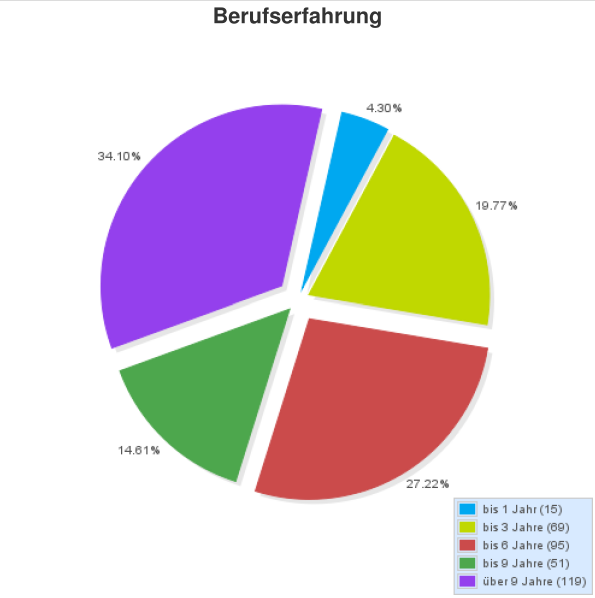
\includegraphics{./material/pie_chart.png}
 % pie_chart.png: 1584x1542 pixel, 72dpi, 55.88x54.40 cm, bb=
 \caption{Beispiel des Designs von Flotr2 Diagrammen}
 \label{fig:pie_chart_flotr}
\end{figure}

\section{Datensicherheit}
Bei der Planung wurde im Vorfeld großes Augenmerk auf die Datensicherheit gelegt und somit als wichtiger Punkt in die Entwicklung einbezogen. Der Grund für einen solchen Punkt ist der, dass mit sensiblen Kundendaten verfahren wird und keiner der Kunden durch eventuelle Datenlücken oder ähnliches diskreditiert werden darf.
Ein Beispiel für solche Daten wird der Student nachfolgend beschreiben: 
Teilnehmer A aus Stadt X nimmt als Einziger aus Stadt X bei der Umfrage teil. Teilnehmer B kennt Teilnehmer A und weiß von ihm, dass er an dieser Umfrage teilnimmt. Nun kann Teilnehmer B Gehaltspannen von Teilnehmer A ablesen, weil die Auswertungen St\"adte basiert sind. Zum Schutz dieser Daten sollte ein Algorithmus implementiert werden, der genau diese Art von Offenlegung von Teilnehmern unterbinden muss. Dieser pr\"uft zuerst wie viele Teilnehmer einer Stadt vorhanden sind. Bei weniger als 3 Teilnehmern wird der Standort in der Auswertung nicht angezeigt. Wenn mindestens drei Teilnehmer aus einer Stadt kommen wird als n\"achstes gepr\"uft, ob insgesamt 15 abgegebene Antworten einer Frage vorhanden sind. Ist dies nicht der Fall wird der Standort auch nicht angezeigt. Mittels dieses Algorithmus' wird verhindert, dass Daten von Teilnehmern offengelegt werden.